\section{Large Catapults in Momentum Gradient Descent}
\label{sec:catapults}

\subsection{Motivating Example: Linear Diagonal Networks}
\label{sec:ldn}

% The diagonal neural network \citep{woodworth2020kernel,pesme2021sgd,nacson2022stepsize} as it is arguably the simplest 
% \cite{woodworth2020kernel} showed that for gradient flow, the scale of initialization induces a separation between kernel and rich regimes; in the latter regime, the algorithm displays sparsity-inducing $\ell_1$ regularization; \cite{nacson2022stepsize} empirically showed that for gradient descent with finite step-size, the scale of the step-size induces a similar separation; \cite{pesme2021sgd} quantified the implicit regularization due to stochasticity when stochastic gradient flow is used.
The linear diagonal network (LDN) is known to be one of the simplest non-linear models that display rich and non-trivial implicit bias~\citep{woodworth2020kernel} while still being mathematically tractable.
Here, we focus on the depth-2 linear diagonal network defined by
\begin{equation}
    f(\vx; \vu, \vv) := \langle \vu \odot \vu - \vv \odot \vv, \vx \rangle 
    %= \langle \vw, \vx \rangle
    , \quad \vx, \vu, \vv \in \sR^d,
\end{equation}
where $\vx$ is the input vector, $(\vu, \vv)$ are the trainable parameters, and $\vw := \vu \odot \vu - \vv \odot \vv$ is the linear coefficient vector.
% In sparse regression problems where the true $\vw$ is assumed to be sparse, it is known that gradient-based optimization has an implicit regularization effect for LDNs that interpolates between minimum $\ell_1$ and $\ell_2$-norm solutions, depending on the scale of initialization \citep{woodworth2020kernel}.

\paragraph{Implicit Bias of LDN.} The training dynamics and implicit bias of the LDN have been rigorously investigated in the literature. Still, most works focus on the continuous regime with vanishing learning rate, such as the (stochastic) gradient flow~\citep{woodworth2020kernel,azulay2021initialization,moroshko2020initialization,pesme2023hopping,pesme2021sgd}.
Although \cite{papazov2024momentum} and \cite{lyu2024momentum} study the impact of momentum on training dynamics, they also focus on the flow regime, which cannot capture phenomena such as the edge of stability or catapults that are inherently unique to the large learning rate regime.
% \cite{papazov2024momentum} derive implicit regularization terms specifically for LDNs trained with momentum gradient flow whereas our phenomenon holds more generally with various architectures, loss, and datasets.  
Recently, there has been some progress for (S)GD with finite step sizes~\citep{nacson2022stepsize,even2023diagonal}, but they do not consider momentum at all.

\citet{woodworth2020kernel} prove that for the sparse regression problem where the true $\vw_\star$ is assumed to be sparse, the gradient flow for LDN initialized at $\vu_0 = \vv_0 = \alpha\cdot\bm{1}$ converges to the minimum $\ell_1$-norm solution as $\alpha \rightarrow 0$ and minimum $\ell_2$-norm solution as $\alpha \rightarrow \infty$.
It is well-known that the minimum $\ell_1$-norm solution has a better generalization capability, due to sparsity of $\vw_\star$.
% If the underlying problem has an intrinsic sparse structure (i.e., if the ground-truth $\vw_*$ is sparse), the minimum $\ell_1$-norm solution has a better generalization capability.
Subsequently, \cite{nacson2022stepsize} show that GD with finite learning rate consistently recovers solutions with smaller test loss, even for initializations with large $\alpha$'s, as shown in Figure~\ref{fig:LDN-gd}.
% Since the properties of vanilla GD are well-known in LDNs, it is only natural to first consider the effect of momentum and learning rate warmup in LDNs to get a clear picture.

\vspace{-5pt}
\paragraph{Experimental Setting.}
We investigate the implicit bias effect of momentum in linear diagonal networks by adding momentum to the sparse regression experiment in \citet{nacson2022stepsize}.
% $\vy_i \sim \gN_d(\langle \bm\theta^\star, \vx_n \rangle, \sigma^2 \mI)$
Throughout this section, we mostly follow their experimental settings.
The training set is $\{(\vx_n, \vy_n)\}_{n=1}^N$ generated as $\vx_n \sim \gN(\bm\mu, \sigma^2 \mI_d)$ and $\vy_n = \langle \vw_\star, \vx_n \rangle$, where $N = 50, \sigma^2 = 5, d = 100, \bm\mu = 5\cdot\bm{1}$ and $\vw_\star = (\delta_{i \leq 5} / \sqrt{5})_i$.
We use the mean squared error (MSE) loss, and we initialize $\vu_0 = \vv_0 = \alpha\cdot\bm{1}$, where $\alpha \in [0, 0.3]$ is the initialization scale.
% For each $\eta_f \in \{ 1 \cdot 10^{-4}, 2 \cdot 10^{-4}, 4 \cdot 10^{-4}, 7 \cdot 10^{-4}, 1 \cdot 10^{-3}, 1.3 \cdot 10^{-3}, 1.8 \cdot 10^{-3}, 2.4 \cdot 10^{-3}, 3.2 \cdot 10^{-3}, 4.2 \cdot 10^{-3}, 5.6 \cdot 10^{-3}, 7.5 \cdot 10^{-3} \}$, 
Following \cite{nacson2022stepsize}, for each $\eta_f$, we use linear warmup (linearly increasing the learning rate) for the first $\eta_f \cdot 10^6$ steps, starting from $\eta_i = 10^{-8}$.
For the momentum parameter of PHB, we use $\beta = 0.9$.

\begin{remark}[Learning Rate Warmup]
    Learning rate warmup is a standard practice in deep learning~\citep{goyal2017warmup}, with known benefits such as variance reduction~\citep{gotmare2018warmup,liu2020warmup} and preconditioning~\citep{gilmer2022stability}.
    We and \cite{nacson2022stepsize} consider learning rate warmup to avoid possible instabilities from using large learning rates.
\end{remark}
% ,goyal2017warmup

% In this paper, we mainly consider linear learning rate warmup, henceforth referred to as ``linear warmup.''

%, which is the default parameter for PyTorch implementation of PHB\footnote{One subtle different is that in the PyTorch implementation the effective momentum coefficient is $\beta \eta$, not $\beta$. Here, we follow the PHB formulation as discussed in \cite{sutskever2013momentum} - \eqref{eqn:momentum}.}.
% In the flow regime ($\eta = ?$), the ``speed'' of implicit bias, i.e., speed of test loss decreasing as one decreases $\alpha$, is faster for PHB than GD, but overall they behave similarly.
% Things are very different for a finite learning rate regime ($\eta = ?$).
% \subsection{Momentum Changes the Implicit Bias of LDN }
\paragraph{Results.}
Over the varying initialization scales $\alpha$ and (final) learning rates $\eta_f$, we report the final resulting test losses in Figure~\ref{fig:LDN}.
Note the striking difference between (a) GD and (b) PHB.
Compared to GD, whose final test loss saturates after some $\alpha$ as reported in \citet{nacson2022stepsize}, it is clear that
\begin{center}
    {\it PHB displays a fundamentally different implicit bias in the large learning rate regime.}
\end{center}
For PHB, the final test loss initially increases monotonically as $\alpha$ increases like GD. However, once $\alpha$ becomes larger than some threshold $\bar{\alpha}(\eta_f)$ (dependent on $\eta_f$), the test loss sharply drops close to zero.
% This phase transition is absent when the LDN is trained using GD.
We also note that $\bar{\alpha}(\eta_f)$ appears to decrease as $\eta_f$ increases.\footnote{In fact, we can see in Figure~\ref{fig:LDN-main-phb} that the final test loss slightly increases (in a noisy fashion) with $\alpha$ after the sharp drop at $\bar \alpha(\eta_f)$. We attribute this phenomenon to \emph{overshooting}; see Appendix~\ref{app:overshooting} for more discussion.}
% Compared to GD, which displays a rather monotonic relationship between $\alpha$ and test loss, i.e., larger $\alpha$ roughly corresponds to larger test loss (up to saturation), it seems clear that in the presence of warmup, PHB has a fundamentally different behavior from GD in the finite learning rate regime.

% {\color{red}\bf One can hypothesize that due to enlarging MSS, adding momentum sometimes averts a catapult that is beneficial to the performance. Thus it is favored that the work can give more discussions and criterions of how adding momentum changes catapults and when momentum helps test performance. Besides, theoretical insights on the effects of initialization scales is also favored.}



\begin{figure*}[!t]
\centering
\subfigure[GD]{
\includegraphics[width=0.43\textwidth]{LDN/sec2_gd_testloss_vs_alpha.pdf}
\label{fig:LDN-gd}
}
\subfigure[PHB]{
\includegraphics[width=0.43\textwidth]{LDN/sec2_phb_testloss_vs_alpha.pdf}
\label{fig:LDN-main-phb}
}

\subfigure[GD Sharpness]{
\includegraphics[width=0.225\textwidth]{LDN/sec2_sharpness_vs_alpha_gd.pdf}
\label{fig:LDN-sharpness-gd}
}
\subfigure[GD Train Loss]{
\includegraphics[width=0.225\textwidth]{LDN/sec2_train-loss_vs_alpha_gd.pdf}
\label{fig:LDN-train-loss-alpha-gd}
}
\subfigure[PHB Sharpness]{
\includegraphics[width=0.225\textwidth]{LDN/sec2_sharpness_vs_alpha_phb.pdf}
\label{fig:LDN-sharpness-phb}
}
\subfigure[PHB Train Loss]{
\includegraphics[width=0.225\textwidth]{LDN/sec2_train-loss_vs_alpha_phb.pdf}
\label{fig:LDN-train-loss-alpha-phb}
}

\caption{Experiments following the same setting as \citet{nacson2022stepsize}. In (a) and (b), "$\ell_1$ baseline" and "$\ell_2$ baseline" respectively stand for the solution with the minimal $\ell_1$ norm and the solution with the minimal $\ell_2$ norm to the regression problem. We use $\beta=0.9$ for PHB.}
\label{fig:LDN}
\end{figure*}


\paragraph{Momentum Induces Larger Catapults.}
% \subsection{Momentum with LR Warmup Induces Greater Sharpness Reduction}
% To further investigate our phenomenon, we need to recall that there are emergent phenomena in the large learning regime. %\citet{cohen2021stability} show that PHB exhibits unstable behaviors when the sharpness exceeds the MSS $\frac{2(1 + \beta)}{\eta}$.
% Indeed, it is known that when the learning rate is sufficiently large such that the iterates' sharpness goes \emph{above} the MSS, then several interesting phenomena such as edge of stability \citep{cohen2021stability} and catapult~\citep{lewkowycz2020catapult} arise, as discussed earlier.
% Throughout this paper, we refer to \emph{catapult} as a sharp increase in loss, followed by a decrease that forms a single spike in the training loss, coupled with a rapid sharpness reduction.

To find the cause for our observed phenomena, we plot the evolution of sharpness for PHB in Figure~\ref{fig:LDN-sharpness-phb} at the $\alpha$ and $\eta$ at which the test loss suddenly drops.
Note that as the warmup proceeds, the MSS decreases monotonically, and as soon as the sharpness of the iterates ``touches'' the MSS curve, it goes through a rapid sharpness reduction, coupled with a loss spike (Figure~\ref{fig:LDN-train-loss-alpha-phb}).
The sharpness reduction of PHB is so drastic that the final sharpness is well below the MSS of the final learning rate.
This is in contrast to GD which goes through an incremental, step-wise sharpness reduction (Figure~\ref{fig:LDN-sharpness-gd}) with multiple loss spikes (Figure~\ref{fig:LDN-train-loss-alpha-gd}), and the final sharpness stays just below the MSS corresponding to the final learning rate; this phenomenon for SGD was also observed in \citet{zhu2023catapult}.
Here, one could make an educated guess that momentum induces much larger catapults that bias the solution towards flatter minima.

One observation is that momentum does not improve test loss over GD across \emph{all} settings (e.g., initialization), as shown in Figure~\ref{fig:LDN-main-phb}. A possible explanation is since the MSS $\frac{2(1+\beta)}{\eta}$ for PHB is higher than the MSS $\frac{2}{\eta}$  of GD with the same $\eta$, the $\alpha$ that causes a catapult for GD may not for PHB, resulting in no improvement, but if a catapult does occur, the sharpness reduction is much more drastic for PHB than GD. With this observation in mind, from this point on, whenever we compare the trajectory of GD and PHB starting from the same initialization, we always match the MSS of GD and PHB by properly rescaling the momentum learning rates $\eta_{PHB} = (1+\beta) \eta_{GD}$ for fair comparison. We only specify the GD learning rate in the text as $\eta$.

\begin{remark}[Role of Warmup in Large Catapults]
\label{rmk:roleofwarmup}
    Although we used linear warmup schedule in the experiments, warmup is not a strict requirement for (large) catapults to occur.
    Indeed, we observe that catapults consistently occur as long as (1) the iterate is initially close to a global minimum and (2) the learning rate is large enough so that the sharpness is slightly above the MSS but small enough so that the iterates do not completely diverge.
    Linear warmup provides a natural way to satisfy these two criteria, whereas 
    using large constant learning rates from the beginning usually results in severe instability.
    %It is difficult to satisfy these two conditions without using warmup, as training with a large constant learning rate from the beginning results in severe instability.
    We remark that one could use different scheduling to induce the catapults; see Appendix~\ref{app:warmup-necessity} for ablations on different warm-up schedules.  
\end{remark}




\begin{figure*}[!t]
    \centering
    \subfigure[Width-200 FCN, $\eta_i=0.001$, $\eta_f=0.05$]{
        \includegraphics[width=0.29\textwidth]{figures/fc-relu/cifar10-1k/w200_lr0.001-0.05_warmup1000/sharpness.pdf}
    }
    \hfill
    \subfigure[Width-1000 FCN, $\eta_i=0.01$, $\eta_f=0.1$]{
        \includegraphics[width=0.29\textwidth]{figures/fc-relu/cifar10-1k/w1000_lr0.01-0.1_warmup200/sharpness.pdf}
    }
    \hfill
    \rulesep
    \subfigure[Width-100 FCN, $\eta_i=0.001$, $\eta_f=0.4$]{
    \includegraphics[width=0.29\textwidth]{figures/fc-relu/cifar10-1k/ce_w100_lr0.001-0.4_warmup500/sharpness.pdf}
    } \\
    \subfigure[Width-1000 FCN, $\eta_i=0.001$, $\eta_f=0.02$]{
        \includegraphics[width=0.29\textwidth]{figures/fc-relu/cifar10-5k/w1000_lr0.001-0.02_warmup500/sharpness.pdf}
    }
    \hfill
    \subfigure[Width-7000 FCN, $\eta_i=0.001$, $\eta_f=0.01$]{
        \includegraphics[width=0.29\textwidth]{figures/fc-relu/cifar10-5k/w7000_lr0.001-0.01_warmup500/sharpness.pdf}
    }
    \hfill
    \rulesep
    \subfigure[Width-200 FCN, $\eta_i=0.001$, $\eta_f=0.05$]{
    \includegraphics[width=0.31\textwidth]{figures/fc-relu/cifar10-5k/ce_w200_lr0.001-0.05_warmup500/sharpness.pdf}
    }
    \caption{Neural Networks trained on (a-c) 1k and (d-f) 5k subset of CIFAR10~\citep{krizhevsky2009learning}.
    For (a,b,d,e), we use the MSE loss, and for (c,f) we the CE loss.
    All FCNs are 3-layer and use ReLU activation. The shaded region is the linear warmup period. 
    }
    \label{fig:cifar10-exp}
\end{figure*}


\subsection{Nonlinear Neural Networks}
\label{sec:modern-arch}
% We perform additional experiments on a 3-layer fully connected ReLU network (FCN) with a synthetic dataset and a ResNet20 with a subset of the CIFAR10 dataset; full experimental details are deferred to Appendix~\ref{app:modern}.
To show that the phenomenon is not limited to LDNs, we also conduct experiments with narrow and wide fully-connected networks (FCN) on 1k and 5k-datapoint subsets of CIFAR10~\citep{krizhevsky2009learning} for both MSE {\it and} cross entropy (CE) losses.
The results are shown in Figure~\ref{fig:cifar10-exp}. It is clear that the catapults observed in PHB reduce the sharpness farther below the MSS than GD. It can also be observed that PHB is more ``sensitive'' to instability, in that sharpness being slightly above the MSS quickly causes catapults; this is in contrast to GD, where the sharpness sometimes hover above the MSS curve. % (2) the catapults observed in PHB dynamics reduces the sharpness farther below the MSS than GD.
%the large catapults occur across various considered settings.
The late-phase dynamics of CE experiments look different from MSE, because sharpness eventually decreases. This can be attributed to the fact that CE loss drives the iterates to flatter region once the model achieves 100\% training accuracy. Even in the case of CE, PHB displays a large drop of sharpness at the moment the sharpness curve touches the MSS curve.
% Notably, the sharpness of GD in the MSE experiments remains close to the MSS throughout training, going through the edge of stability~\citep{cohen2021stability} and highly unstable training. In contrast, the sharpness of PHB displays large catapults, resulting in the final sharpness stabilizing well below the MSS. 
Additional experiments, including results for ResNet20 and for $\beta = 0.99$, can be found in Appendices~\ref{app:modern} and \ref{app:099}.
% {\color{red}\bf CJHECK ADD}
















% \begin{figure}[!t]
%     \centering
%     \subfigure[Step warmup.]{
%         \includegraphics[width=0.45\linewidth]{figures/step-warmup/lr0.0023_Twarmup10000_alpha0.2/u^2-v^2_hess-sharpness.pdf}
%         \label{fig:ldn-step-warmup}
%     }
%     \subfigure[Terminating the warmup.]{
%         \includegraphics[width=0.45\linewidth]{figures/warmup_stop/lr0.005_Twarmup5000_Twarmupstop2150_alpha0.2/u^2-v^2_hess-sharpness.pdf}
%         \label{fig:warmup-stop}
%     }
%     \caption{Ablations on the learning rate warmup. (a) Step warmup is used instead of linear warmup. (b) The warmup period is initially set to $5000$ iterations, but the warmup is terminated at iteration $2150$ around the iteration where the sharpness crosses the MSS.}
%     \label{fig:ldn-warmup}
% \end{figure}

% % {\color{red} Another observation is that with PHB, no PS is observed after a large catapult, while with GD, PS is often observed (Figure~\ref{fig:LDN-sharpness-gd} and \ref{fig:LDN-sharpness-phb}).
% % To see why this is the case, in Figure~\ref{fig:ldn-coordinates}, we plot the evolution of the coordinates $\vw_t^{(i)}$ of the linear coefficient vector $\vw_t := \vu_t \odot \vu_t - \vv_t \odot \vv_t$.
% % We observe that the large catapults in PHB result in a {\it sparsification effect}, in which the non-support coordinates of the ground-truth $\vw_*$ are forced down to almost zero and become stationary afterwards.
% % GD, on the other hand, has a much less sparsification effect, and the coordinates continue to change even after each catapult.}
% % }

% % \begin{figure}[!th]
% %     \centering
% %     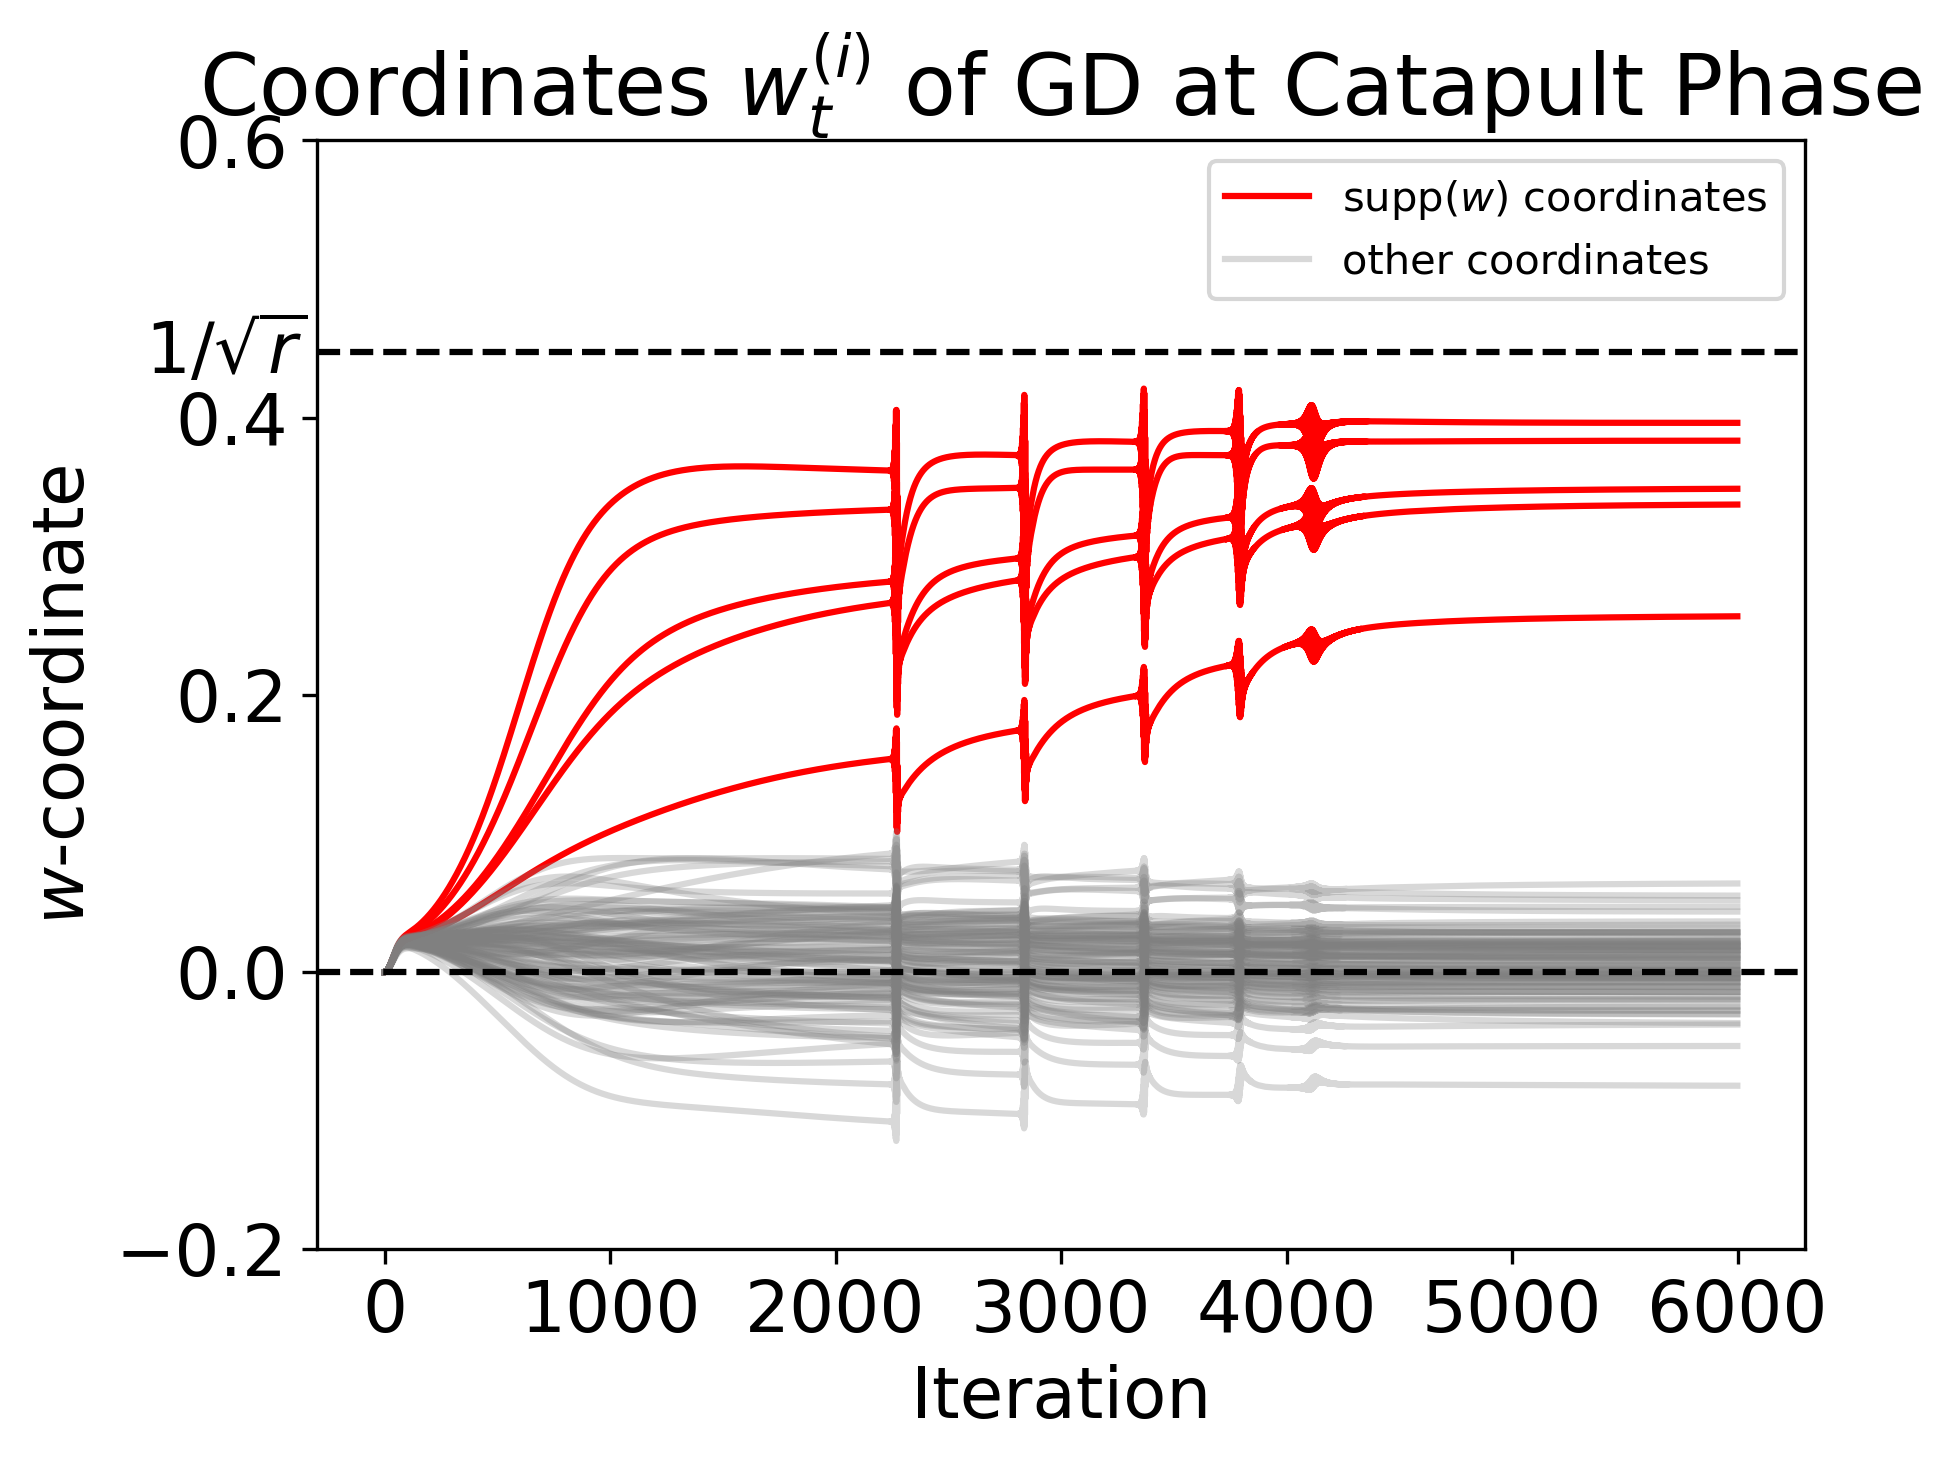
\includegraphics[width=0.49\linewidth]{figures/ldn_coordinates_0.0.png}
% %     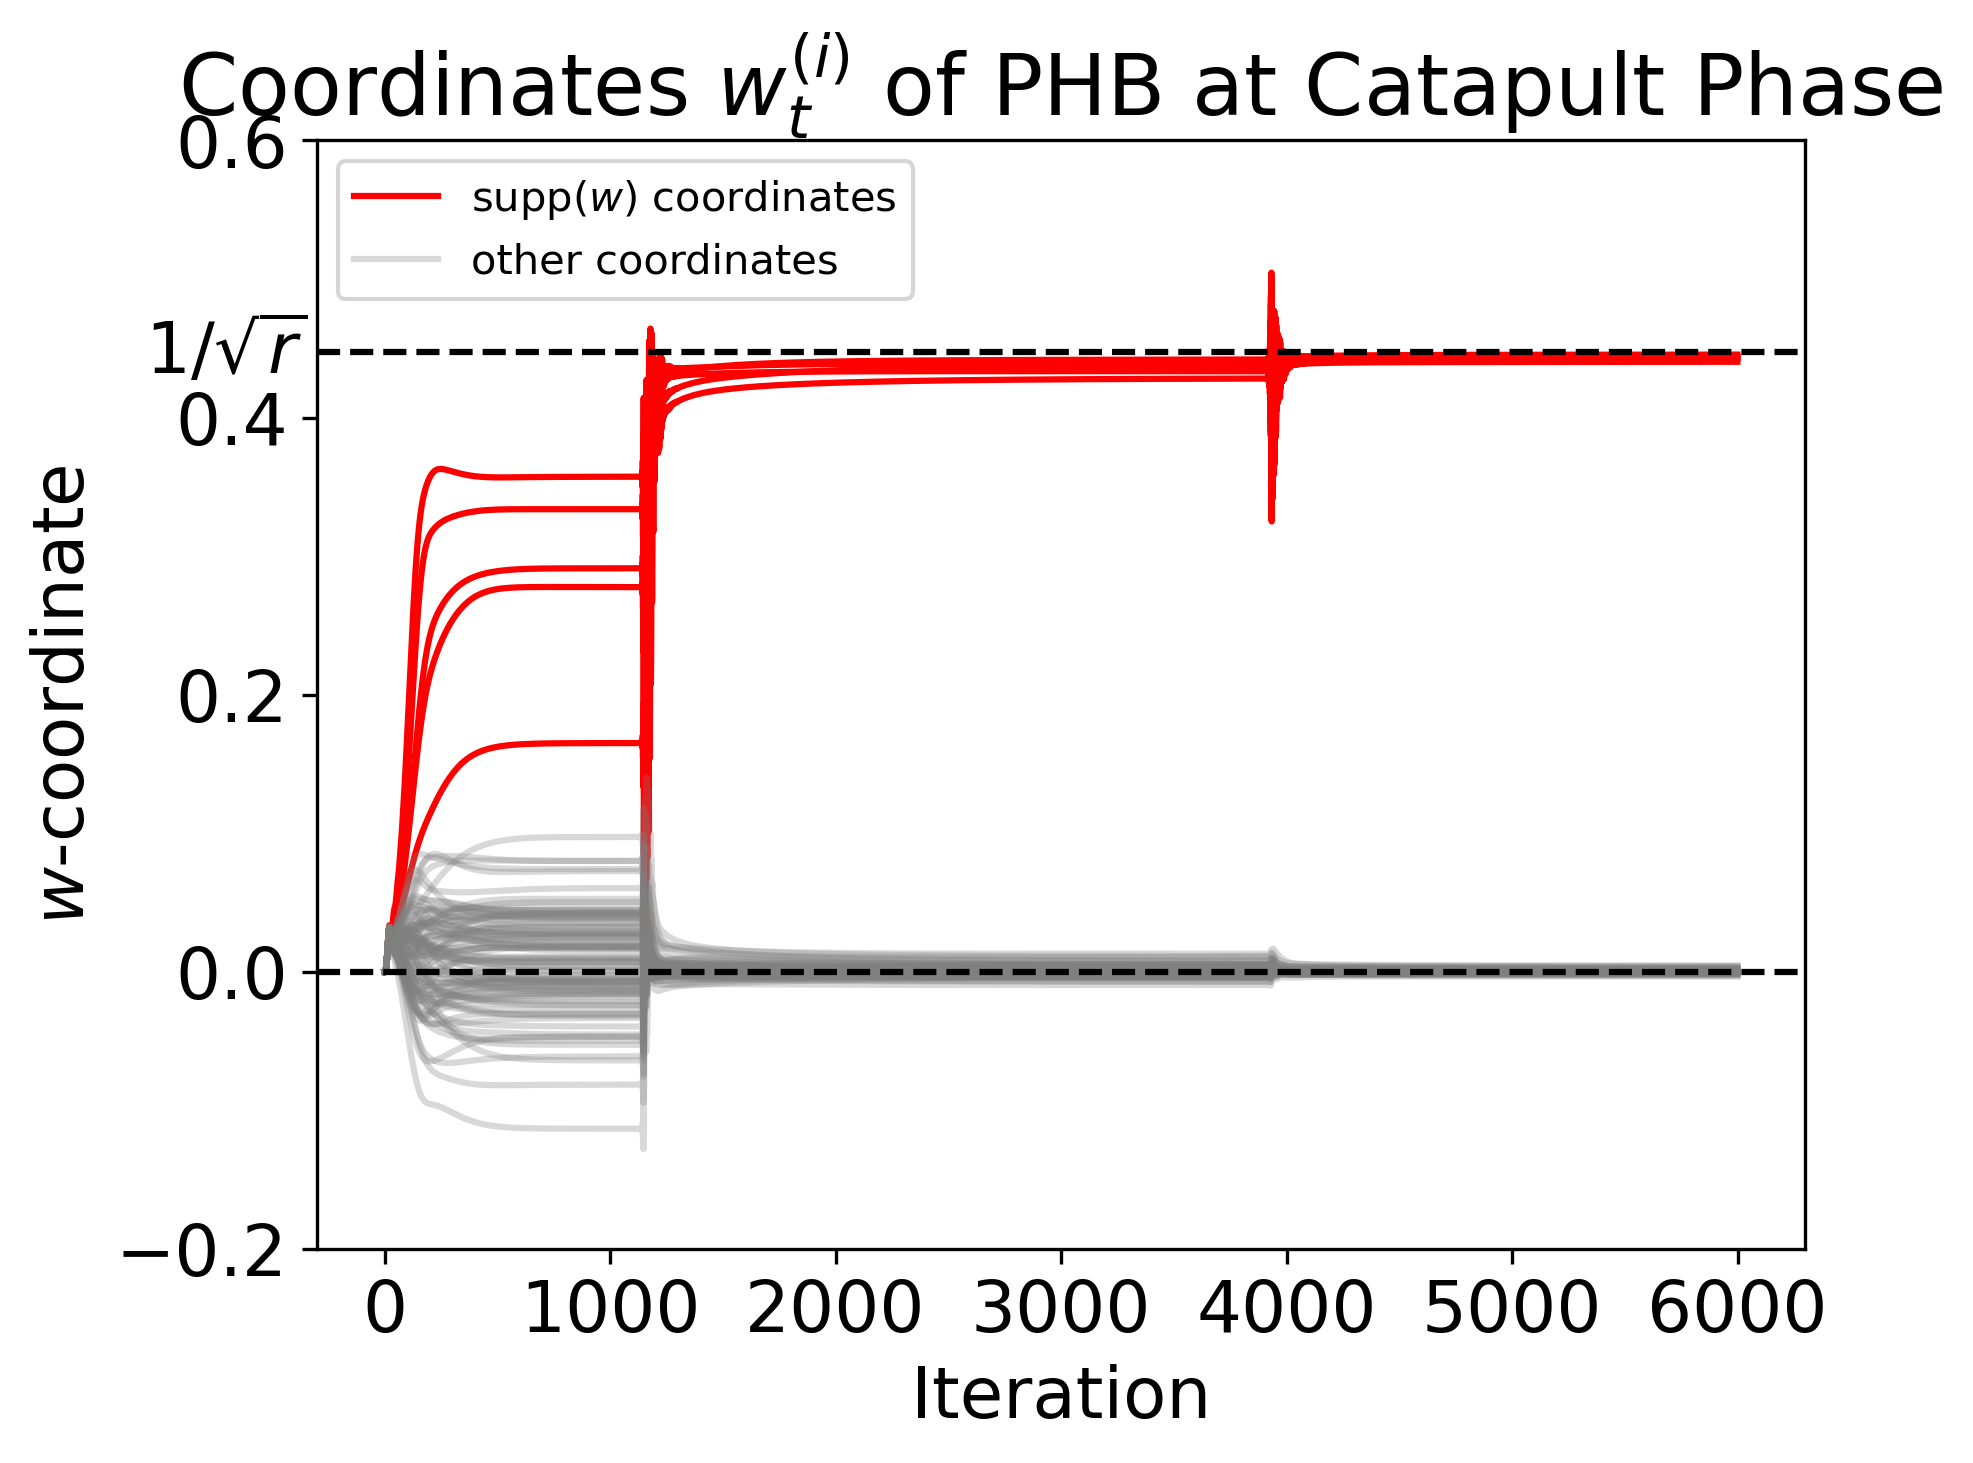
\includegraphics[width=0.49\linewidth]{figures/ldn_coordinates_0.9.png}
% %     \caption{Evolution of coordinates of $\vw$ for GD (left) and PHB (right). The setting is the same with our LDN experiment in Section~\ref{sec:ldn}, except we set $\eta_f = 0.015$ and $T_{warmup} = 4000$. This aggressive schedule is to emphasize the sparsification effect of large catapults.
% %     {\color{red} make BIGGER}
% %     }
% %     \label{fig:ldn-coordinates}
% % \end{figure}



% \subsection{Is Linear Warmup Necessary?}
% \label{subsec:warmup-necessity}
% Although we use linear warmup in our experiments, we emphasize that linear warmup is {\it not} necessary to induce the catapults.
% We observe that the main criteria for inducing the catapults are (1) for the iterates to be in a neighborhood of a stable minimum and (2) for the current learning rate to be large enough that the minimum is unstable (in that the sharpness of the minimum is above the MSS) but not so unstable that training diverges.
% % and are (1) convergence to an initial (sharp) minimum and (2)
% Linear warmup satisfies these two criteria by (1) stably moving the iterates towards a minimum under a low learning rate and (2) automatically finding a suitably large learning rate (that does not lead to divergence) by gradually increasing the learning rate. However, as long as the two criteria are met, catapults can be induced without linear warmup.

% To show that the specific form of the warmup is not essential in inducing the catapults, we train an LDN using a step warmup scheduler.
% We use the learning rate of $10^{-5}$ for the first $10000$ iterations and then $0.0023$ for the remaining $10000$ iterations. Here, it is necessary to use a sufficiently long warmup period to ensure that the pre-catapult training loss is close to zero. 
% % Note that under the same learning rate, the MSS of GD and PHB differ by a factor of $(1+\beta)$.
% Since both GD and PHB are initialized at the same $\alpha \cdot \bm{1}$, the learning rate used for the PHB experiment is the specified learning rate multiplied by $(1+\beta)$ to match the MSS and ensures that if the sharpness hits the MSS for GD, it also hits the MSS for PHB.
% As shown in Figure~\ref{fig:ldn-step-warmup}, this setting also induces a catapult despite not using linear warmup.
% It should be noted that, unlike linear warmups, the final learning rate must be carefully tuned to prevent training from diverging. 
% %We can interpret step warmup as a two-phase process of (1) finding a stable minimum by training under low $\eta$ and then (2) inducing a catapult by using a constant but sufficiently large $\eta$.
% %{\color{red}Notably, this suggests that if the parameters are initialized close to a minimum and $\eta$ is initialized so that the initial sharpness is only slightly above the MSS, large catapults can be induced while keeping $\eta$ constant as in the second phase of step warmup. Based on this observation, we consider a constant (but large) $\eta$ setting to simplify the analysis in Section \ref{sec:prolong}.}
% % (unlike linear warmup, which ``smoothly'' leads to a point that induces catapults): if the learning rate is too small, the catapult is not induced, and if it is too large, training diverges.

% To show the effectiveness of the linear warmup in finding the appropriate scale of the learning rate for inducing catapults, we terminate the warmup as soon as the sharpness crosses the MSS, even before the prescribed warmup period ends.
% As shown in Figure \ref{fig:warmup-stop}, this is enough to induce catapults for PHB, supporting our claim that linear warmup has the advantage of ``smoothly'' finding a suitable learning rate for inducing catapults.









% {\color{red}
% We want to directly compare to the experiments of \citet{even2023diagonal}
% \begin{enumerate}
%     \item Evolution of the coordinates of $\bm\beta$
%     \begin{itemize}
%         \item If $\bm\beta$ is sparse, then catapults have a somewhat ``sparsifying'' effect (as in LDN, near the minima, sharpness roughly corresponds to infinity-norm; see \cite{even2023diagonal}).
%         This effect is amplified with momentum.

%         \item {\bf (Hypothesis)} If $\bm\beta$ is not sparse but there exists a sparse $\bm\beta'$ that fits the training data, then the LDN converges to the sparser one and thus has a simplicity bias?
%     \end{itemize}

%     \item Test loss, {\it two} sharpness measures ($\lambda_{max}(\nabla^2)$ and $\tr(\nabla^2)$) w.r.t. varying stepsize and momentum parameter.

%     \item What if the stochastic version is used? It is known that stochasticity has a benign implicit bias in LDNs~\cite{even2023diagonal,pesme2021sgd}.

%     \item simulate semi-theory equations using LDN (compare different terms, e.g. $\nabla E \cdot \nabla \lambda_0$, $(\theta_{t-2}-\theta_{t-3}) \cdot \nabla \lambda_0$
% \end{enumerate}

% {\bf How does catapult fit in with all the phenomena? What about with momentum?}
% \begin{itemize}
%     \item edge of stability~\citep{cohen2021stability}

%     \item homegeinty effect

%     \item ...etc?
% \end{itemize}
% \begin{enumerate}
%     \item Try to show an interpolation between EoS and catapult
%     \begin{itemize}
%         \item convergence -> EoS -> catapult -> divergence, as we change the stepsize/initialization (turning a single knob)

%         \item No EOS?? No progressive sharpening??

%         \item (Prin) Momentum GD is {\it qualitatively} different from GD
%     \end{itemize}
% \end{enumerate}


% Deep learning experiments:
% \begin{enumerate}
%     \item (Bohan) Can the acceleration effect be linked to a catapult?
%     With a large stepsize, the catapult reduces sharpness, after which the sharpness increases.
%     The duration of the increase can roughly correspond to acceleration?

%     \item 
% \end{enumerate}

% }


% is a suitable choice for finding the right learning rate for inducing the catapults. By gradually increasing the learning rate, warmup is able to find a sufficiently large learning rate that induces catapults but not one that is so large as to cause the parameters to diverge.




% \begin{figure}[h]
%     \centering
%     \includegraphics[width=0.32\textwidth]{figures/step-warmup/lr0.00225_Twarmup1000_alpha_0.2/u^2-v^2_train-loss_zoomed.pdf}
%     \includegraphics[width=0.32\textwidth]{figures/step-warmup/lr0.00225_Twarmup1000_alpha_0.2/u^2-v^2_test-loss_zoomed.pdf}
%     \includegraphics[width=0.32\textwidth]{figures/step-warmup/lr0.00225_Twarmup1000_alpha_0.2/u^2-v^2_hess-sharpness.pdf}
%     \caption{Linear Diagonal Network trained using step warmup}
%     \label{fig:ldn-step-warmup}
% \end{figure}


% \begin{figure}[ht]
%     \centering
%     \includegraphics[width=0.32\textwidth]{figures/warmup_stop/lr0.005_Twarmup5000_Twarmupstop2150_alpha0.2/u^2-v^2_train-loss_zoomed.pdf}
%     \includegraphics[width=0.32\textwidth]{figures/warmup_stop/lr0.005_Twarmup5000_Twarmupstop2150_alpha0.2/u^2-v^2_test-loss_zoomed.pdf}
%     \includegraphics[width=0.32\textwidth]{figures/warmup_stop/lr0.005_Twarmup5000_Twarmupstop2150_alpha0.2/u^2-v^2_hess-sharpness.pdf}
%     \caption{Linear Diagonal Network trained using learning rate warmup. The warmup period is initially set to 5000 iterations, but warmup is terminated at iteration 2150 around the iteration where the sharpness crosses the MSS.}
%     \label{fig:warmup-stop}
% \end{figure}